% !TEX root = ../main.tex
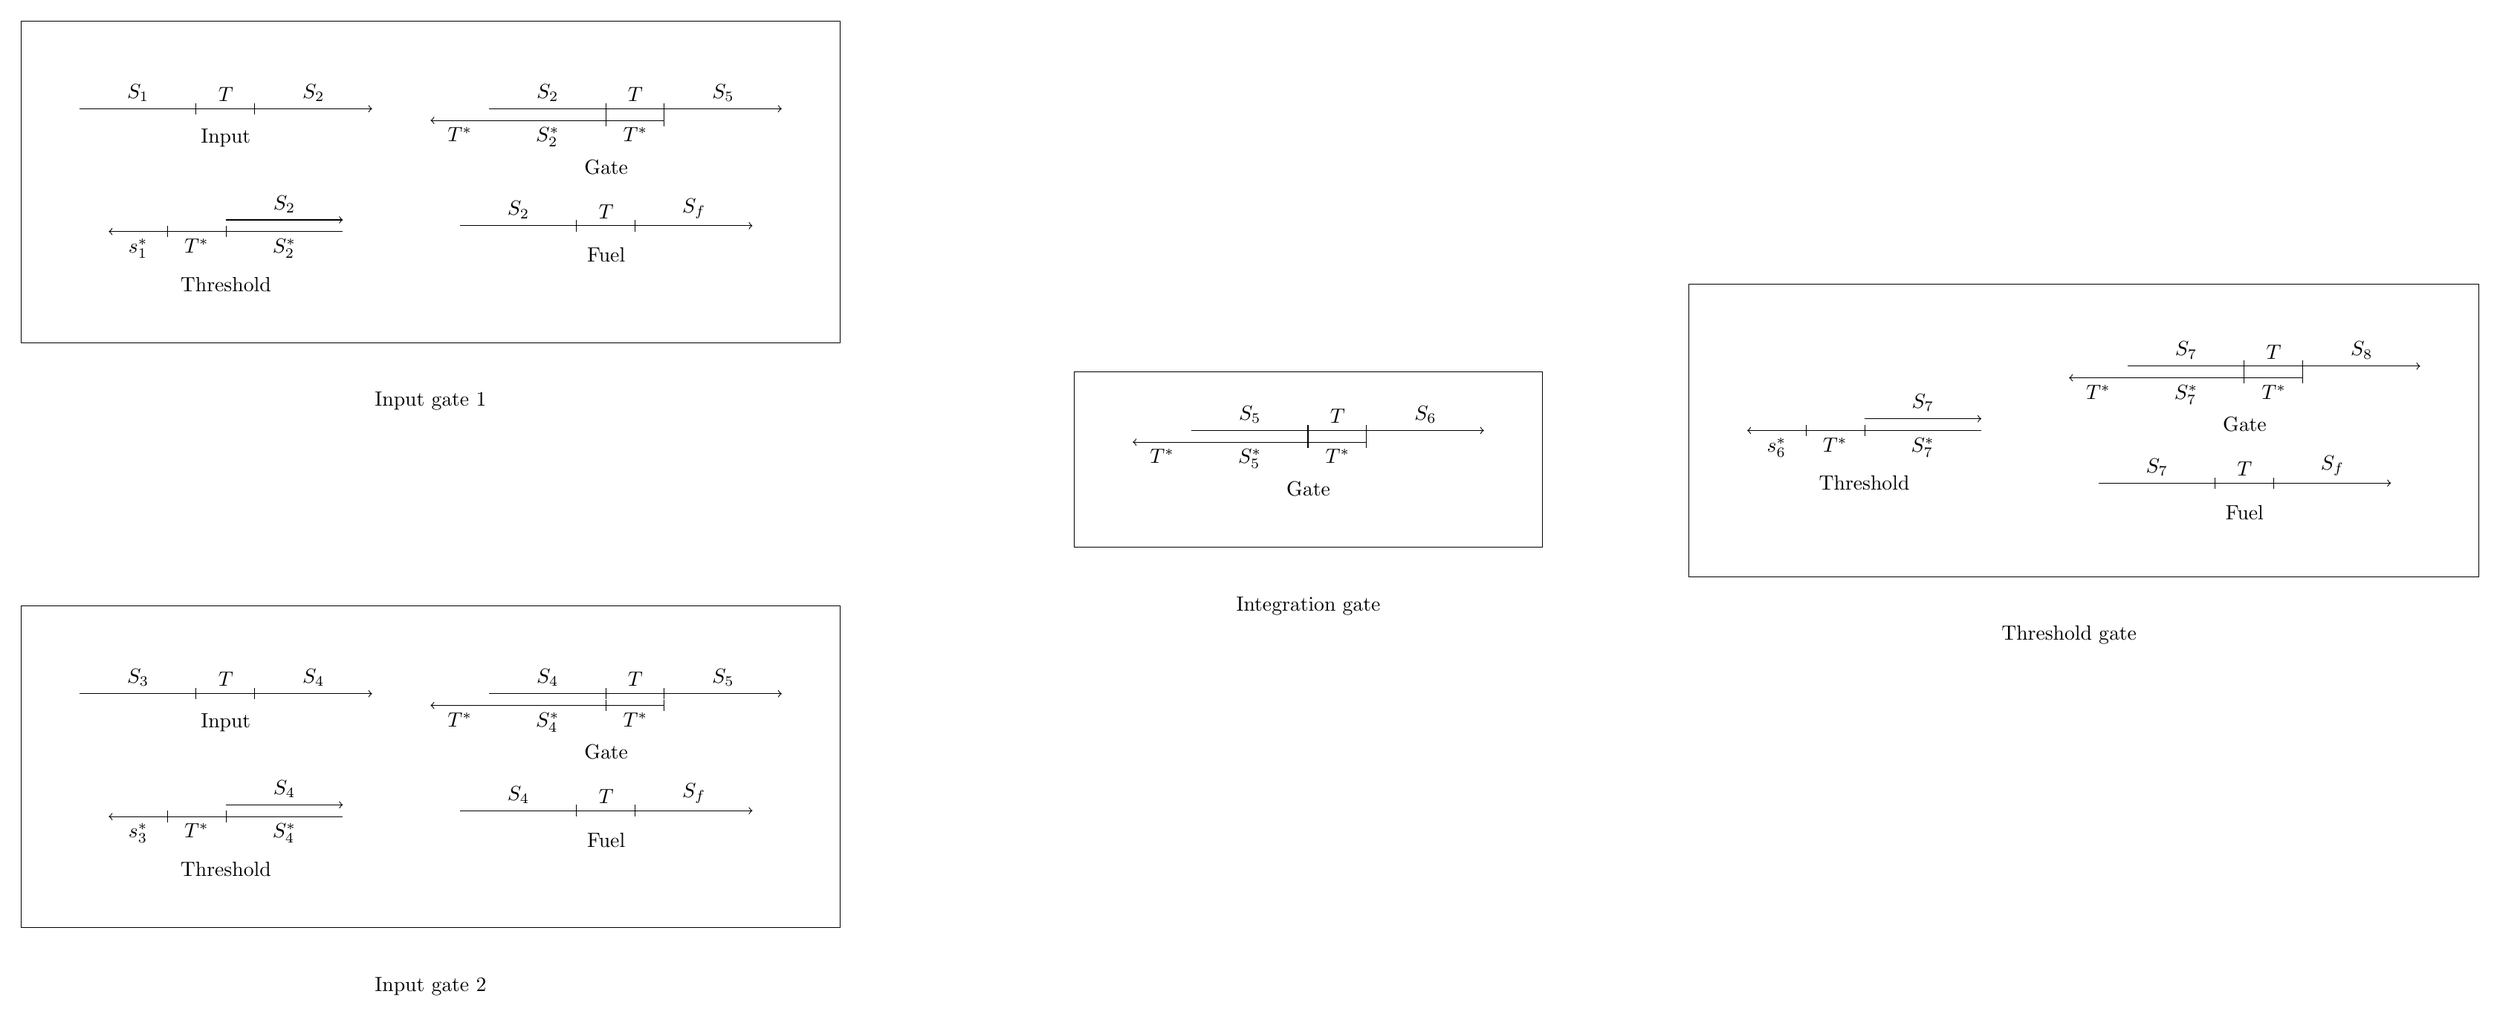
\begin{tikzpicture}

\def\gate(#1,#2,#3,#4){

  \begin{scope}[shift={(#1,#2)}]
    \draw[-|](8, -1.5) -- node[above] {$#3$} (10, -1.5);
    \draw[-|](10, -1.5) -- node[above] {$T$} (11, -1.5);
    \draw[->](11, -1.5) -- node[above] {$#4$} (13, -1.5);

    \draw[<-](7, -1.7) -- node[below] {$T^*$} (8, -1.7);
    \draw[-|](8, -1.7) -- node[below] {$#3^*$} (10, -1.7);
    \draw[-|](10, -1.7) -- node[below] {$T^*$} (11, -1.7);
    \node[align=center] at (10, -2.5) {Gate};
\end{scope}
}

\def\threshold(#1,#2,#3,#4,#5){
  \begin{scope}[shift={(#1,#2)}]
    \draw[<-](7, -0.1) -- node[below] {$#5^*$} (8, -0.1);
    \draw[|-](8, -0.1) -- node[below] {$T^*$} (9, -0.1);
    \draw[|-](9, -0.1) -- node[below] {$#4^*$} (11, -0.1);
    \draw[->](9, 0.1) -- node[above] {$#4$} (11, 0.1);
        \node[align=center] at (9, -1) {Threshold};
  \end{scope}
}

\def\fuel(#1,#2, #3){
  \begin{scope}[shift={(#1,#2)}]
\draw[-|](0, -3) -- node[above] {$#3$} (2, -3);
\draw[-|](2, -3) -- node[above] {$T$} (3, -3);
\draw[->](3, -3) -- node[above] {$S_f$} (5, -3);

\node[align=center] at (2.5, -3.5) {Fuel};
\end{scope}
}

\def\inputstrand(#1,#2, #3, #4){
  \begin{scope}[shift={(#1,#2)}]
    \draw[-|](0, 0) -- node[above] {$#3$} (2, 0);
    \draw[-|](2, 0) -- node[above] {$T$} (3, 0);
    \draw[->](3, 0) -- node[above] {$#4$} (5, 0);

    \node[align=center] at (2.5, -0.5) {Input};
  \end{scope}
}

\def\inputgate(#1,#2, #3, #4,#5, #6){
  \begin{scope}[shift={(#1,#2)}]

    \gate(#1-1,#2+1.5, #4, #5);
    \threshold(#1-6.5,#2-2, #3, #4, #6);
    \fuel(#1+6.5,#2+1, #4);
    \inputstrand(#1,#2, #3, #4);
  \end{scope}
}

\def\thresholdgate(#1,#2, #3, #4,#5, #6){
  \begin{scope}[shift={(#1,#2)}]

    \gate(#1-1,#2+1.5, #4, #5);
    \threshold(#1-6.5,#2-1, #3, #4, #6);
    \fuel(#1+6.5,#2+1, #4);
  \end{scope}
}

\inputgate(0, 0, S_1, S_2, S_5, s_1);


\inputgate(0, -5, S_3, S_4, S_5, s_3);

\gate(11, -4, S_5, S_6);

\thresholdgate(14, -2.2, S_6, S_7, S_8, s_6);

\draw (-1, 1.5) rectangle (13, -4);
    \node[align=center] at (6, -5) {Input gate 1};


\draw (-1, -8.5) rectangle (13, -14);
    \node[align=center] at (6, -15) {Input gate 2};


\draw (17, -4.5) rectangle (25, -7.5);
    \node[align=center] at (21, -8.5) {Integration gate};

\draw (27.5, -3) rectangle (41, -8);

    \node[align=center] at (34, -9) {Threshold gate};


% \gate(0, 0, S_2, S_3);
% \threshold(0, -4, S_1, S_2, s_1);
% \fuel(0, -8, S_2);
% \inputstrand(0, 0, S_1, S_2);

\end{tikzpicture}
